\chapter{光的粒子性}\label{chp:particle_light}
光的电磁说使光的波动理论发展到相当完美的地步,取得了巨大成就。
但是,这个学说并不能完美地解释所有的光现象,还在赫兹用实验证实光的电磁说的时候,就已经发现了后来叫做光电效应的现象,这个现象使光的电磁说遇到了无法克服的困难。
二十世纪初,人们在新的事实的基础上建立了关于光的新的学说——光子说,对光的本性的认识又前进了一步。

\section{光电效应}
\par\medskip\noindent
\begin{minipage}{0.52\linewidth}\parindent2em
1887 年,赫兹在进行电磁波的实验时发现了一个奇妙的现象:当紫外线照射到圆环接收器间隙的电极上时,火花放电变得容易了。
后来其他科学家又发现,用紫外线照射与验电器相连的带负电的锌板时,验电器的金箔便立即闭合。
用紫外线照射与验电器相连的不带电的锌板时,验电器上带正电。
通过这些现象人们认识到,用紫外线照
\end{minipage}\hfill
\begin{minipage}{0.45\linewidth}
\begin{figurehere}
  \includegraphics{7-1.pdf}
  \caption{紫外线照射锌板使验电器带正电}\label{fig:7-1}
\end{figurehere}
\end{minipage}
\par\vskip6pt\noindent
射金属时,电子会从金属表面飞出来。
在紫外线照射下,赫兹实验中的电极变得容易放电,带负电的锌板失去电荷,不带电的锌板带上了正电,都是由于电子从金属表面飞出来了的缘故。

在光的照射下物体中发射电子的现象,叫做\Concept{光电效应}。
光电效应中发射出来的电子叫做\Concept{光电子}。
实验表明,不仅紫外线能产生光电效应,对于碱金属,例如锂、钠、钾、铯等,用可见光照射也能产生光电效应。
\begin{figure}
  \includegraphics{7-2.pdf}
  \caption{研究光电效应的装置简图}\label{fig:7-2}
\end{figure}

\cref{fig:7-2} 是研究光电效应规律的实验装置简图。
其中 $S$ 是抽成真空的容器,$C$ 是石英窗口,紫外光和可见光都可以通过它射到容器里的金属板 $K$ 上。
在 $K$ 的对面有另一金属板 $A$,$K$ 和 $A$ 组成一对电极。
象图中那样把 $K$ 跟电池组的负极相连,$A$ 正极相连。
电路接好后,电流表指示没有电流,因为极板 $K$ 和 $A$ 之间是断开的。
用一定强度的光照射极板 $K$,它发射出的光电子运动到极板 $A$ 时,电流表的指针就发生偏转,指出电路中产生了电流。
这电流是由光电子产生的,叫做光电流。

逐渐增加极板 $K$ 和 $A$ 间的正向电压(使 $A$ 板电势比 $K$ 板高),电路里的光电流也逐渐增大。
当正向电压增到几伏时,光电流就达到最大值——饱和值。
再增加电压,光电流也不再增大了。
这表明 $K$ 板发射的光电子已全部被 $A$ 板吸去。
这时增加入射光的强度,光电流值就继续上升。
入射光的强度增加一倍,光电流的饱和值也增加一倍,这表明,\emph{在单位时间里从极板 $K$ 发射出的光电子数跟入射光的强度成正比}。

逐渐减小极板 $K$ 和 $A$ 间的正向电压,当这电压减小为零时,电路里仍有相当强的光电流。
可见光电子从极板 $K$ 飞出时具有某种初动能,没有正向电场的作用,也有相当数量的光电子到达极板 $A$。
要完全阻止光电流,必须在 $KA$ 间加一定的反向电压(使 $A$ 板电势低于$K$板电势),使那些具有最大初动能的光电子不足以克服反向电场的阻力而到达极板 $A$,就没有光电流了。
这时,光电子的最大初动能 $\frac{1}{2}mv^2_m$ 与反向电压 $U$ 之间有下面的关系:
\[\dfrac{1}{2}mv^2_m=eU, \]
式中的 $e$ 表示电子的电量。
因此,从实验中测出使光电流减小到零时的反向电压 $U$ 的值,就可以求出光电子的最大初动能。
实验表明,\emph{光电子的最大初动能与入射光的强度无关,只随着入射光频率的增大而增大}。

换用不同材料的极板 $K$ 重做实验,结果表明,光电子的最大初动能还跟极板 $K$ 的材料有关。
\emph{对于任何一种金属,入射光的频率必须大于某一极限频率才能产生光电效应;低于这个极限频率的光,无论强度如何,照射时间多长,也不能产生光电效应}。
\cref{tab:7-1} 是几种金属的极限频率 $\nu_0$ 和波长 $\lambda_0$。
\begin{table}
  \caption{几种金属的极限频率 $\nu_0$ 和波长 $\lambda_0$}\label{tab:7-1}
  \begin{tblr}{colspec={X[c]X[r]X[2,r]X[c]X[r]X[2,r]},hline{2}=0.8pt,vline{4}=1.2pt,row{1}={m,c}}
    金属& $\lambda_0$(\unit{\micro m})& $\nu_0$(\unit{Hz})& 金属& $\lambda_0$(\unit{\micro m})& $\nu_0$(\unit{Hz})\\
    铯&0.66&  $ \num{4.545e14}$ &    钠 & 0.50 &  $ \num{6.000e14}$ \\
    锌&0.37&  $ \num{8.065e14}$ &    银&0.26&  $ \num{1.153e15}$ \\
    铂& 0.20& $ \num{1.529e15}$ &      &    &              \\
  \end{tblr}
\end{table}

\section{爱因斯坦对光电效应的解释}
\subsection{光子}
光电效应的规律无法用经典的波动理论来解释。
按照波动理论,光的能量是由光的强度决定的,而光的强度又是由光波的振幅决定的,跟频率无关。
因此,不论光的频率如何,只要光的强度足够大或照射时间足够长,都应该有足够的能量产生光电效应,然而这跟实验结果是直接矛盾的。
极限频率的存在,即频率低于某一数值的光不论强度如何都不能产生光电效应,这是波动理论不能解释的。

对光电效应的解释是 1905 年爱因斯坦(1879--1955)在普朗克(1858--1947)的量子论的基础上作出的。
1900 年德国物理学家普朗克在研究电磁辐射的规律时发现,只有假设电磁辐射的能量是不连续的,而是一份一份地进行的,每一份的能量是 $h\nu$,其中 $\nu$ 是辐射的频率,是一个普适恒量,理论计算的结果才能跟实验事实很好地符合。
这个 $h$ 后来就叫做\Concept{普朗克恒量},实验测出 $h=\qty{6.63e-34}{J.s}$。
在普朗克的量子说的启发下,爱因斯坦天才地预见到,为了解释光电效应必须假设光也是不连续的,而是一份一份的,每一份光叫做一个\Concept{光子},光子的能量跟它的频率成正比,即 $E=h\nu$,其中的 $h$ 是普朗克恒量。
这就是爱因斯坦在 1905 年提出的光子说。
爱因斯坦是在实验事实还不很充分的情况下做出这一假设的,但是从这个假设得出的一切结论都跟后来的实验结果相符。

光子说很好地解释了光电效应。
当光子照射到金属上时,它的能量可以被金属中的某个电子全部吸收,电子吸收光子的能量后,动能就增加了。
如果电子的动能足够大,能够克服内部原子对它的引力,就可以离开金属表面逃逸出来,成为光电子,这就是光电效应。
电子吸收光子的能量后可能向各个方向运动,有的向金属内部运动,并不出来。
向金属表面运动的电子,经过的路程不同,途中损失的能量也不同,因此从表面出来时的初动能也不同。
只有直接从金属表面出来的光电子才具有最大初动能,这些光电子克服金属原子的引力所做的功叫做\Concept{逸出功}。
根据能量守恒定律,光电子的最大初动能跟入射光子的能量 $h\nu$ 和逸出功 $W$ 之间有下面的关系:
\[\frac{1}{2}mv^2_m=h\nu-W.\]
这个方程叫做爱因斯坦\Concept{光电效应方程}。

对于一定的金属来说,逸出功 $W$ 的值是一定的。
所以,入射光子的频率 $\nu$ 越大,光电子的最大初动能也越大,如果入射光子的频率比较低,它的能量小于金属的逸出功,就不能产生光电效应了。
这就是存在极限频率的原因。
极限频率 $\nu_0$ 可由下式求出:
\[h\nu_0=W\quad \Rightarrow\quad \nu_0=\frac{W}{h}. \]

不同金属的逸出功不同,所以它们的极限频率也不同。
如果入射光比较强,即单位时间内入射光子的数目多,产生的光电子也多,所以光电流的饱和值也大。

\begin{Practice}
\begin{question}
  \item 使锌板产生光电效应的光子的最长波长是 \qty{0.37}{\micro m},这种光子的能量是多少电子伏?锌的逸出功是多少?
  \item 可见光的光子,能量范围是多大(用电子伏表示)?为什么用可见光不能使锌板产生光电效应?
  \item 铯的逸出功是 \qty{3.0e-19}{J},用波长是 \qty{0.59}{\micro m} 的黄光照射铯,电子从绝表面飞出的最大初动能是多大?
  \item 钨的逸出功是 \qty{4.52}{eV},使钨产生光电效应的最长波长是多少?这种波长是可见光吗?
\end{question}
\end{Practice}

\section{光电效应的应用}

利用光电效应可以把光信号转变为电信号,动作迅速灵敏,因此利用光电效应制作的光电器件在工农业生产,科学技术和文化生活领域内得到了广泛的应用。
光电管就是应用最普遍的一种光电器件。

光电管的类型很多。
\cref{fig:7-3a} 是其中的一种,玻璃泡里的空气已经抽出,有的管里充有少量的惰性气体(如氩、氖、氦等),管的内半壁涂有逸出功小的碱金属作为阴极 $K$。
管内另有一阳极 $A$。
使用时照\cref{fig:7-3b} 那样把它连在电路里,当光照射到光电管的阴极 $K$ 时,阴极发射电子,电路里就产生电流。
光电管不能受强光照射,否则容易老化失效。
光电管产生的电流很弱,应用时可以用放大器把它放大。
\begin{figure}
  \begin{minipage}[b]{0.45\linewidth}\centering
    \includegraphics{7-3a.pdf}
    \subcaption{}\label{fig:7-3a}
  \end{minipage}
  \begin{minipage}[b]{0.45\linewidth}\centering
    \includegraphics{7-3b.pdf}
    \subcaption{}\label{fig:7-3b}
  \end{minipage}
  \caption{光电管}\label{fig:7-3}
\end{figure}

下面举例说明光电管的应用。

\subsection{光控继电器}
工业生产中的大部分光电控制设备都用光控继电器。
\cref{fig:7-4} 是光控继电器的示意图。
它由电源、光电管、放大器、电磁继电器几部分组成。
当光照射光电管时,光放大器电管电路中便产生电流,经放大器放大后,使电磁铁 $M$ 磁化,把衔铁 $N$ 吸住;没有光照射光电管时,电路中没有电流,衔铁 $N$ 在弹簧的作用下就自动离开 $M$。
如果把衔铁 $N$ 跟控制机构相连,就可以达到自动控制的目的。
\begin{figure}
  \includegraphics{7-4.pdf}
  \caption{光控继电器示意图}\label{fig:7-4}
\end{figure}

光控继电器在工业上可以用于产品的自动计数、安全生产等方面。
用于自动计数时,可以把产品放在传送带上,光源和光电管分别放在传送带的两侧,每当传送带上输送过去一个产品时,光线被挡住一次,光控继电器就放开衔铁一次,由衔铁控制的计数器的数字就加一。
工人在冲床、钻床、锻压机械上劳动时,如有不慎,容易出事故。
为保证安全,可以在这些机床上安装光控继电器,当工人不慎将手伸人危险部位时,由于遮住了光线,光控继电器就立即动作,使机床停下来,避免事故的发生。

\subsection{有声电影}
最早的电影是没有声音的。
后来虽然有了声音,但那是靠留声机来配合影片播放的。声和影配合不好时,效果当然不好。
我们现在能够看到声和影完全配合一致的有声电影,还是多亏了光电管。

影片摄制完后,要进行录音。
录音时通过专门的设备使声音的变化转变成光的变化,从而把声音的“像”摄制在影片的边缘上,形成宽窄变化的暗条纹,这就是影片边上的\Concept{音道}。

放映电影时,利用光电管把“声音的照片”还原成声音。
方法是:在电影放映机中用强度不变的极窄的光束照射音道,由于影片上各处的音道宽窄不同,所以在影片移动的过程中,通过音道的光的强度也就不断变化;变化的光射向光电管时,在电路中产生变化的电流,把电流放大后,通过喇叭就可以把声音放出来。

\section{光的波粒二象性}
光的干涉、衍射和偏振等现象无可争辩地表明光具有波动性,而光电效应又无可争辩地表明光是具有能量 $E=h\nu$ 的光子流,也就是说光具有粒子性。
这样,已经退出历史舞台的光的微粒说,在二十世纪初又以新的形式被重新提了出来。
当然人们现在对光的粒子性的认识比起十七世纪牛顿提出微粒说时已经大不相同。
人类对光的本性的认识经过曲折的发展过程已经越来越深入了。
现在,人们认识到,光既具有波动性,又具有粒子性,也就是说,\emph{光具有波粒二象性}。

十七世纪的微粒说和波动说是互相对立的两种学说,都企图用一种观点去说明光的本性,这是受了传统观念的影响。
传统观念是我们在观察周围世界的宏观现象中形成的,波动性和粒子性在宏观现象中是互相对立的、矛盾的,没有任何宏观物体既有波动性、又有粒子性。
对于宏观物体来说,波粒二象性是不可想像的。

但是,对于光子这样的微观粒子,却只有从波粒二象性出发,才能说明它的各种行为。
实际上,光子说并没有否定光的电磁说,光子的能量 $E=h\nu$,其中的频率 $\nu$ 表示的仍是波的特征。
此外,从光子说和电磁说还往往得到一致的结论。
例如,光子说和电磁说都可以推导出光具有动量,并且为实验所证实。
光子说的结论是光子的动量 $p=h\nu/c$,电磁说的结论是辐射能 $E$ 具有的动量是 $p=E/c$。
由于光子的能量 $E=h\nu$,所以从这两个学说得到的结论是一致的,由于 $c=\lambda\nu$,光子的动量也可以写成
\[p=\frac{h}{\lambda},\]
式中的波长 $\lambda$ 表示的也是波的特征。
可见,对于宏观物体来说不可想像的波粒二象性,在微观世界却是不可避免地必须予以承认的现实。接受光的波粒二象性,就要求我们既不可把光当成宏观观念中的波,也不可把光当成宏观观念中的粒子。

那么,在微观世界中,波和粒子又是怎样统一起来的呢?
物理学家做的下述实验可以帮助我们理解这个问题。
在光的双缝干涉实验中,在像屏处放上照相底片,并设法减弱光流的强度,由于每个光子的能量 $h\nu$ 可以从频率 $\nu$ 算出,因此进一步从光流的能量可以算出所含光子的数目。
这样就可以使光流减弱到使光子只能一个一个地通过狭缝。
实验结果表明,如果曝光时间不太长,底片上只出现一些无规则分布的点子,那些点子是光子打在底片上形成的,表现出光的粒子性。
这些点子的分布是无规则的,可见光子的运动跟我们在研究宏观现象时假设的质点的运动不同,没有一定的轨道。
如果曝光时间足够长,底片上就出现了规则的干涉条纹,就象用强光经短时间曝光后产生的一样。
可见,光的波动性是大量光子表现出来的现象。
在干涉条纹中,那些光波强度大的地方,也就是光子到达机会多的地方,或者说,是光子到达的几率大的地方;光波强度小的地方,是光子到达的几率小的地方。
所以从这种意义上,可以把光的波动性看做是表明大量光子运动规律的一种\Concept{几率波}。

一般说来,大量光子产生的效果往往显示出波动性,个别光子产生的效果往往显示出粒子性,让我们稍稍详细地说明一下。

无线电波的频率较低,波长较长,这种电磁波的“光子”的能量很低,以频率为 \qty{1}{MHz} 的无线电波来说,它的“光子”的能量只有 \qty{4e-9}{eV},能量这样低,只有非常大量的“光子”才能使接收装置发生反应。
较好的接收机大约要每秒收到 \num{e10} 个这样的“光子”才起作用,所以,这部分电磁波的波动性很容易观察到,要观察这部分电磁波的粒子性,觉察个别“光子”的作用,却是非常不容易的。

可见光的频率范围大致是 \qtyrange{4e14}{8e14}{Hz},这种光子的能量大约是几个电子伏。
人造的仪器设备既可以比较容易地探测到大量的这种光子的作用,也可以比较容易地探测到少数这种光子的作用,因此这种电磁波的波、动性和粒子性都能够比较容易地观察到。

随着电磁波频率的增大,波长越来越短,波动性就越来越不显著,而粒子性却越来越明显了。
伦琴射线的光子的能量大约是几千电子伏,$\gamma$ 射线的光子的能量在几兆电子伏以上。
个别 $\gamma$ 射线的光子很容易探测出来,而要看到它们的干涉、衍射现象却很困难了。
伦琴射线只有用晶体作衍射光栅才能看到衍射图样,因为晶体内粒子间的距离恰好是 \qty{e-10}{m} 左右。
至于 $\gamma$ 射线,连用晶体作衍射光栅也不行,因为晶体里粒子间的距离,比它的波长大得不可比拟。

总之,要理解各种频率的电磁波,我们必须综合运用波动的观点和粒子的观点。
而且要注意到,这里的波动并不等同于宏观世界里的机械波,这里的粒子也不等同于宏观世界里的质点。

\section{物质波}
在光具有波粒二象性的启发下,法国物理学家德布罗意(1892--1987)在 1924 年提出一个假说,指出波粒二象性不只是光子才有,一切微观粒子,包括电子和质子、中子,都有波粒二象性。
他把光子的动量与波长的关系式 $p=h/\lambda$ 推广到一切微观粒子上,指出:具有质量 $m$ 和速度 $v$ 的运动粒子也具有波动性,这种波的波长等于普朗克恒量 $h$ 跟粒子动量 $mv$ 的比,即
\[\lambda=\frac{h}{mv}.\]
这个关系式后来就叫做德布罗意公式。

从德布罗意公式很容易算出运动粒子的波长。
例如,电子的电荷是 \qty{1.6e-19}{C},质量是 \qty{0.91e-30}{kg},经过 \qty{200}{V} 电势差加速的电子获得的能量
\[E=Ue=200\times \num{1.6e-19}=\qty{3.2e-17}{J}.\]
这个能量就是电子的动能,即
\[\dfrac{1}{2}mv^2=\qty{3.2e-17}{J}.\]
因此
\[v=\sqrt{\frac{2\times \num{3.2e-17}}{\num{0.91e-30}}}=\qty{8.4e6}{m/s}.\]
于是,按照德布罗意公式这运动电子的波长是
\[\begin{split}
    \lambda=\dfrac{h}{mv}&=\frac{\num{6.63e-34}}{\num{0.91e-30}\times \num{8.4e6}}\,\unit{m} \\
&=\qty{8.7e-11}{m}=\qty{0.87}{\text{\AA}.}
\end{split}\]
我们看到,这个波长与伦琴射线的波长相仿。
前面讲过,这样短的波长,只有用晶体做衍射光栅才能观察到衍射现象。
后来人们的确用这种办法观察到了电子的衍射,从而证明了德布罗意假说的正确性。
\begin{figure}
  \includegraphics{7-5.pdf}
  \caption{电子衍射实验示意图}\label{fig:7-5}
\end{figure}

\cref{fig:7-5} 是一种电子衍射实验的示意图。
从灯丝 $K$ 发射出的电子经过电势差为 $U$ 的加速电场,然后通过一组栏板 $D$ 的小孔,成为很细的电子束射到铝箔 $M$ 上,在铝箔的后面放一张照相底片 $P$。
于是就得到\cref{fig:7-6} 所示的照片,在中央斑点的周围出现了环形的明暗相间的花纹。
这个衍射图样跟伦琴射线穿过同一铝箔后产生的衍射图样(\cref{fig:7-7})非常相似。
这是电子具有波动性的证明。根据铝箔原子间的距离、加速电势差和衍射条纹的几何图形,还可以算出电子衍射时的波长,实测结果跟德布罗意公式相符。

\begin{figure}
  \begin{minipage}[b]{0.48\linewidth}
    \centering
    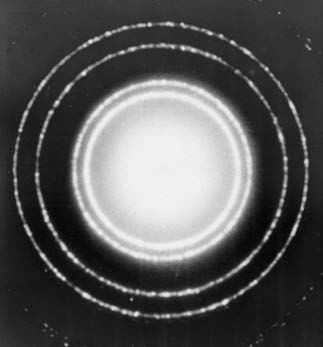
\includegraphics[scale=.8]{7-6.jpg}
    \caption{电子衍射图样}\label{fig:7-6}
  \end{minipage}
  \begin{minipage}[b]{0.48\linewidth}
    \centering
    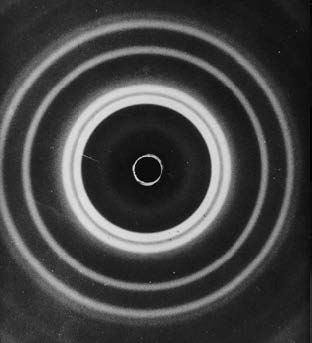
\includegraphics[scale=.8]{7-7.jpg}
    \caption{伦琴射线衍射图样}\label{fig:7-7}
  \end{minipage}
\end{figure}

后来人们又用原子射线和分子射线做类似的实验,同样得到了衍射图样。
质子和中子的衍射实验也做成功了,这就证明了一切运动的微观粒子都具有波粒二象性,其波长与动量的关系都符合德布罗意公式。
于是人们就把这种波叫做德布罗意波或\Concept{物质波}。

那么,物质波是一种什么波呢?
我们知道,机械波是周期性的振动在媒质内的传播,电磁波是周期变化的电磁场的传播。
物质波既不是机械波,也不是电磁波。
在德布罗意提出物质波以后,人们曾经对它提出过各种各样的解释。
到 1926 年,德国物理学家玻恩(1882--1970)提出了符合实验事实的后来为大家公认的统计解释:物质波在某一地方的强度跟在该处找到它所代表的粒子的几率成正比,按玻恩的解释,\emph{物质波乃是一种几率波}。

牛顿力学完全不能解释电子等微观粒子的衍射现象,用物质波的统计解释却很容易说明这种现象。
在\cref{fig:7-5} 的实验里,电子流通过金属箔片以后,物质波发生衍射。
有的地方由于波的叠加而使物质波的强度增大,电子到达这里的几率就大,因而到达这里的电子数较多,有的地方由于波的叠加而使物质波的强度减小甚至等于零,电子到达这里的几率就较小甚至等于零,因面到达这里的电子数很少甚至没有。

发现了电子、质子等微观粒子的波动性以后,我们对微观世界的认识统一起来了。
不但原来认为是电磁波的光具有粒子性,而且原来认为是粒子的电子、质子等也具有波动性。
当然,应该指出,虽然所有的微观粒子都具有波粒二象性,但光子跟电子、质子等粒子还是有很基本的区别的。
光子没有静质量,电子、质子等都有静质量。
光子的运动速度永远是 $c$,电子、质子等却可以有低于光速 $c$ 的各种不同的运动速度。

\begin{Review}
\begin{question}
  \item 什么是光电效应?光电效应有哪些重要的规律?这些规律中哪些是波动说无法解释的?
  \item 什么是光子说?光子说是怎样解释光电效应的?写出光电效应方程
  \item 说明光电管的结构和原理,并举例说明它的应用。
  \item 为什么说光具有波粒二象性?应该怎样理解光的波粒二象性?
  \item 德布罗意提出的物质波的含义是什么?什么实验证明了德布罗意物质波假设的正确性?
\end{question}
\end{Review}

\begin{Exercise}
\begin{question}
  \item 功率为 \qty{1}{W} 的手电筒灯泡大约有 5\% 的电能转化为可见光,试估算它 \qty{1}{s} 能释放出多少个可见光的光子。
  \item 使铜产生光电效应的最低频率是 \qty{1.1e15}{Hz},用频率为\qty{1.5e15}{Hz} 的紫外线照射铜时,它发射出的光电子的最大速度是多大?
  \item 一个质量为 \qty{4e-4}{g} 的尘埃颗粒,以 \qty{1}{cm/s} 的速度在空气中下落,计算它的德布罗意波长。
  \item 计算速度为 \qty{e3}{m/s}的中子的德布罗意波长。这个波长跟 $\gamma$ 射线的波长相比如何?中子的质量是 \qty{1.67e-27}{kg}。
\end{question}
\end{Exercise}